\documentclass{beamer}

\usepackage[square,sort]{natbib}
\setbeamerfont{footnote}{size=\tiny}
\setbeamerfont{footnote mark}{size=\tiny}
\setbeamerfont{caption}{size=\scriptsize}
\setbeamerfont{cite}{size=\tiny}

\usepackage[english]{babel}
\usepackage[utf8]{inputenc}

% AMSLaTeX packages
\usepackage{amsthm}
\usepackage{amsmath}
\usepackage{amsfonts}
\usepackage[algoruled]{algorithm2e}

\usetheme{default}
\useoutertheme{default}
% we want to use images
\usepackage{graphicx}
\usepackage{movie15}
\usepackage{hyperref}

% table relates packages
\usepackage{booktabs}
\usepackage{multirow}
% pick a font
\usepackage{palatino}           
% \usepackage{times}
\usepackage{tikz}
\usetikzlibrary[positioning,arrows,decorations.pathmorphing,backgrounds,fit,calc]
% \AtBeginSection[]  % "Beamer, do the following at the start of every section"
% {
%   \begin{frame}<beamer> 
%     \frametitle{Outline} % make a frame titled "Outline"
%     \tableofcontents[currentsection]  % show TOC and highlight current section
%   \end{frame}                    
% }

% \AtBeginSubsection[]
% {
%   \begin{frame}
%     \frametitle{Outline}
%     \tableofcontents[currentsection,currentsubsection]
%   \end{frame}
% }

\AtBeginSection[]
{
   \begin{frame}
       \frametitle{Outline}
       \tableofcontents[currentsection]
   \end{frame}
}

\newcommand{\ebox}[1][1em]{\framebox[#1]{\phantom{M}}}

\setlength\arraycolsep{1.4pt}% some length

%gets rid of navigation symbols
\setbeamertemplate{navigation symbols}{}

%gets rid of bottom navigation bars
\setbeamertemplate{footline}[page number]{}
\setbeamertemplate{headline}{}


\usebackgroundtemplate{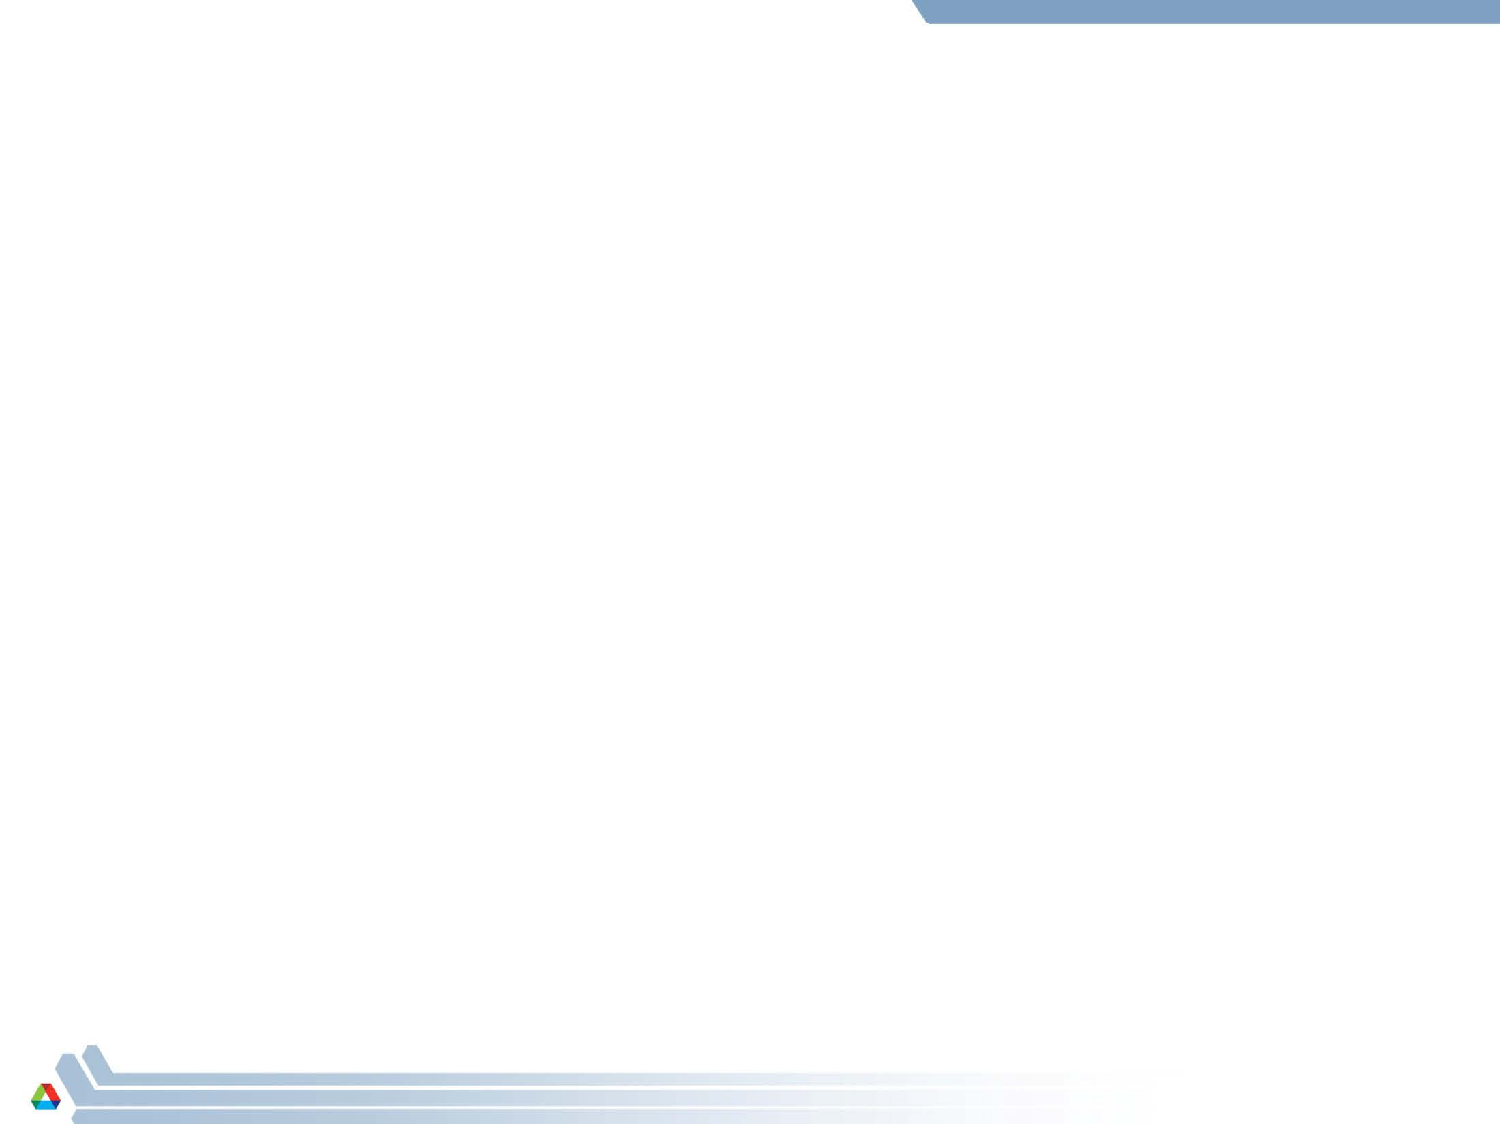
\includegraphics[width=\paperwidth]{NormalANLBlue}}
\title[LANS Seminar]
{Title for the talk}
\author[Speaker]{Author List}
\subtitle{}
\institute[ANL/MCS]{Argonne National Laboratory}
\date{\today}
\begin{document}

\setbeamertemplate{footline}{}
{
\usebackgroundtemplate{
\includegraphics[width=\paperwidth]{TitleANLBlue}}
\frame{\titlepage}
}

\setbeamertemplate{footline}[page number]{total pages}

% FRAME: overview
\begin{frame}
  \frametitle{Outlines}
  \tableofcontents
\end{frame}
% ========================================
% main slides come here
% ========================================

\section{Tomography}
\begin{frame}{Basics}
	\begin{block}{}
		\begin{itemize}
			\item Radon transform : Real $\rightleftarrows$ Sinogram space.
			\item $Rf(\tau,\theta) = 
			\int_{-\infty}^{\infty}\int_{-\infty}^{\infty}
			f(x,y)\delta(\tau - x cos(\theta) - y sin(\theta))dxdy $
		\end{itemize}
	\end{block}
	\begin{center}
		\begin{figure}
			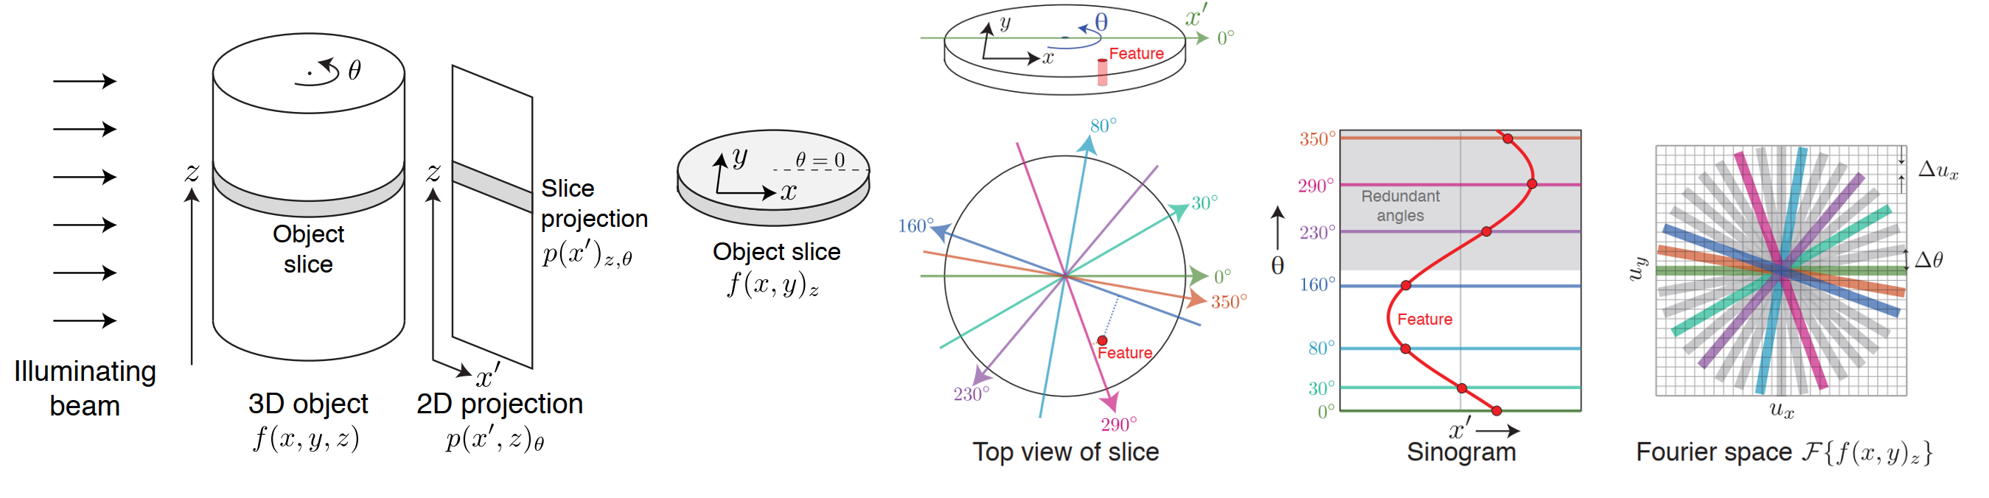
\includegraphics[scale=0.335]{figures/ppa_combined.png}
			\caption{Spinning the object to obatin "sinograms", reconstruct each slice independently\footnote{\cite{jacobsen_2019}}}
		\end{figure}
	\end{center}
	
\end{frame}

\begin{frame}{Center of rotation drifts}
	\begin{columns}[onlytextwidth,T]
		\column{\dimexpr\linewidth-45mm}
		\begin{block}{}
			\begin{itemize}
				\item $P_{\theta} = x_{\theta}^{*}(1-cos(\theta) + y_{\theta}^{*}sin(\theta))$ 
				\item $Rf(\tau,\theta,0,0) = Rf(\tau - P_{\theta},\theta,x_{\theta}^{*},y_{\theta}^{*})$
				\item Translation of sinogram by $P_{\theta}$ achieved by convolution with gaussian.
				\item Recover $P_{\theta}$ to obtain accurate reconstruction!
			\end{itemize}					
		\end{block}
		\column{40mm}
		\begin{figure}
			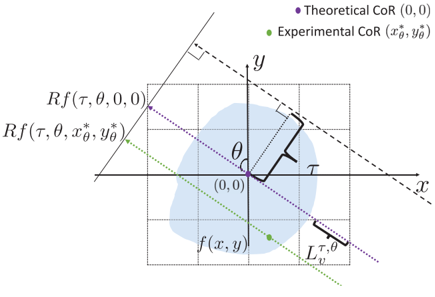
\includegraphics[width=45mm]{figures/drifts.png}
			\caption{Center of rotaion drift causes us to measure the shifted sinograms!}
		\end{figure}
	\end{columns}
\end{frame}

\section{Algorithm}

\begin{frame}{Optimzation formulation}
	\begin{block}{Discretize \& Vectorize}
		\begin{itemize}
			\item $\mathcal{W}$ : object vector
			\item $\mathcal{L}$ : discretized radon transform
			\item $\mathcal{D}$ : measure sinogram
		\end{itemize}
	\end{block}
	\begin{exampleblock}{Least squares cost function}
		\begin{itemize}
			%\item Assuming no shifts, we need
			%$\underset{\mathcal{W} \geq 0}{\textit{min}}  %\frac{1}{2}||\mathcal{L}\mathcal{W}-\mathcal{D}||$
			\item To recover both shifts and object : 
			$\underset{\mathcal{W} \geq 0, P_{\theta}}{\textit{min}}  \phi(\mathcal{W},P_{\theta}) = \frac{1}{2}||\mathcal{L}\mathcal{W} - g(\mathcal{D},P_{\theta})||$
			\item First order derivaties analytically computable :
			$ \nabla \phi(\mathcal{W},P_{\theta}) = [\mathcal{L}^{T},
			\nabla_{P_{\theta}} \phi(\mathcal{W},P_{\theta})] (\mathcal{L}\mathcal{W} - g(\mathcal{D},P_{\theta}))$
		\end{itemize}
	\end{exampleblock}
\end{frame}

\begin{frame}{Implementation}
	\begin{block}{}
		\begin{itemize}
			\item Implemented in C/C++ using :
			\begin{itemize}
				\item PETSc (which handles the optimization routines, data management and parallel I/O)
				\item Boost (which handles geometry routines) 
				\item FFTW (for position correction cost function evaluation).
			\end{itemize}
			
		\end{itemize}
	\end{block}
	\begin{block}{Joint}
		\begin{itemize}
			\item Combine shifts and sample into one vector and optimize for both together.
		\end{itemize}
	\end{block}
	\begin{exampleblock}{Alternating}
		\begin{itemize}
			\item Alternate between optimizing with respect to sample and with respect to shifts.
		\end{itemize}
	\end{exampleblock}
\end{frame}

\section{Results}
\begin{frame}{Accuracy}
	\begin{center}
		\begin{figure}
			\hspace*{-0.5cm}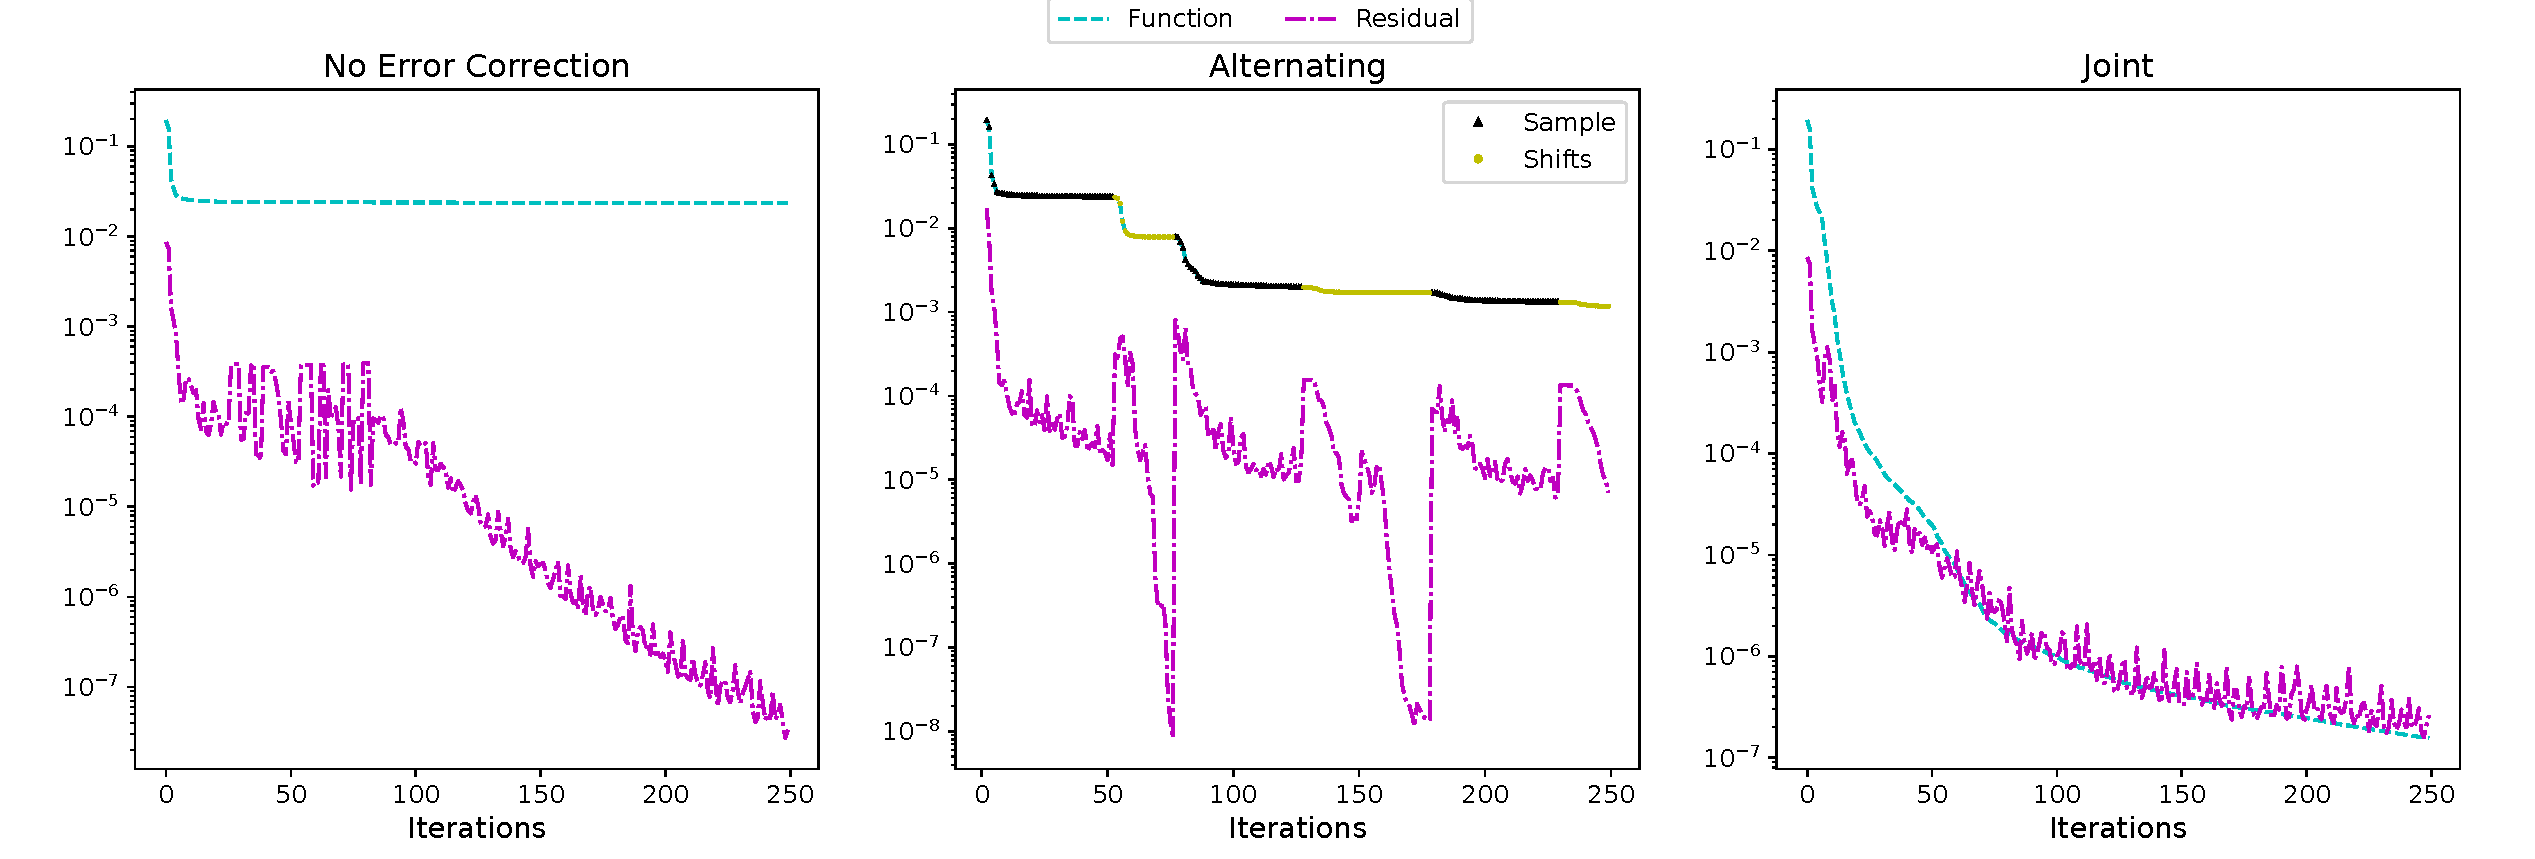
\includegraphics[scale=0.275]{figures/func_resd.pdf}
			\caption{Objective function and gradient norm as a function of iteration number. Dimensions of unknowns : $50+256x256$ and size of experimental data : $256x50$}
		\end{figure}
	\end{center}
\end{frame}
\begin{frame}{Scaling}
	\begin{center}
		\begin{figure}
			\hspace*{-1.5cm}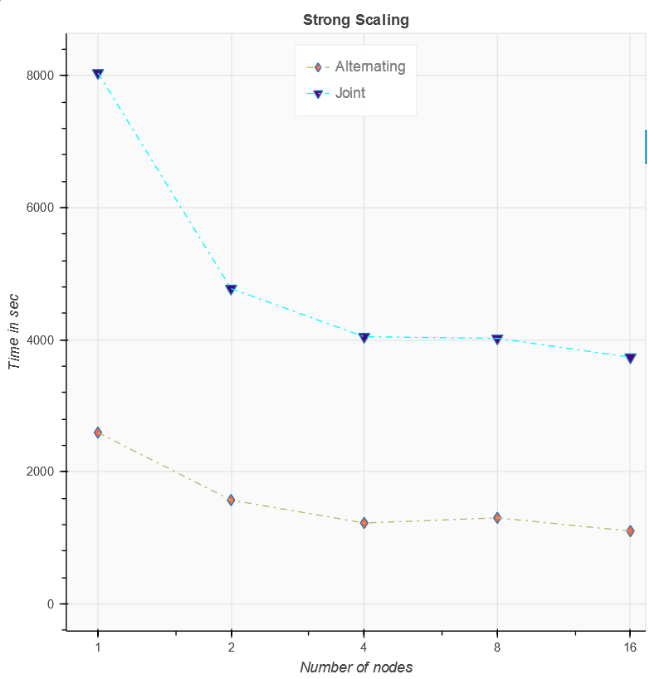
\includegraphics[scale=0.25]{figures/strscale.png}
			\caption{Strong scaling plots for alternating and joint reconstruction algorithms.}
		\end{figure}
	\end{center}
\end{frame}

\section{Future}
\begin{frame}{Next Steps}
	\begin{itemize}
		\item Invert 3D tomography data by replicating the 2D solve on sub-communicators.
		\item Port application to GPU.
	\end{itemize}
\end{frame}

{\usebackgroundtemplate{
		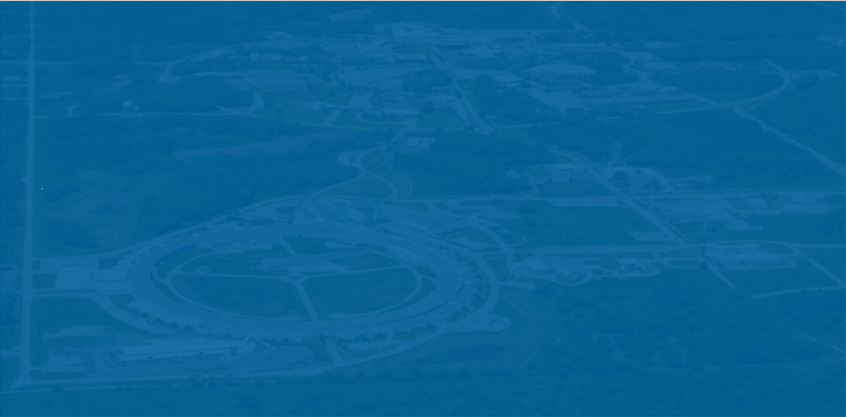
\includegraphics[width=\paperwidth,height=0.9\paperheight]{graphics/closing.png}} 
	\begin{frame}
		\begin{center}
			\begin{itemize}
				\item[] {\Large \textcolor{white}{Thank you!}}
			\end{itemize}			
		\end{center}
		%\vspace{0.3cm}
		%\paragraph{\textbf{\textcolor{white}{Acknowledgements:}}}
		\begin{itemize}
			\item \textcolor{white} {PETSc-Users mailing list.}
		\end{itemize}
	\end{frame}
}
\renewcommand*{\bibfont}{\scriptsize}
\begin{frame}[t, allowframebreaks]
	\frametitle{References}
	\bibliographystyle{dinat-etal}
	\bibliography{pirt}
\end{frame}



\end{document}
